\section {モデルの検証}
	\index{もでるのけんしょう@モデルの検証}
モデルの検証は、VDM++のツールであるVDMToolsを使った場合、以下を行う。

\begin{enumerate}
\item モデルを実行せずにツールで検証する静的検証
\item モデルを実行して検証する動的検証
\end{enumerate}

	\subsubsection {静的検証}
		\addcontentsline{toc}{section}{静的検証}
		\index{せいてきけんしょう@静的検証}
各仕様ファイル毎の構文チェックと、
全仕様ファイルに静的な解析で分かるエラーがないかをチェックする型チェック、
およびツールが生成する証明課題のレビューを行う。

このチェックで、かなりの単純ミスが検出される。

		\paragraph {証明課題レビュー}
		\index{しょうめいかだいれびゅー@証明課題レビュー}
証明課題は、ツールから生成されるVDM++の条件式で、
生成されるすべての条件式がtrueであることが証明できれば、
モデルに内部矛盾が無いことを主張できる。

通常は、条件式がtrueであることを証明するのだが、
開発現場では証明を行うことが難しいので、
生成された証明課題をレビューすることで検証を行う。

証明課題レビューでは、不足する不変条件や事前条件あるいは事後条件が見つかることが多い。

	\subsubsection {動的検証}
		\addcontentsline{toc}{section}{動的検証}
		\index{どうてきけんしょう@動的検証}
VDM++のツール(VDMTools
\footnote{\url{http://fmvdm.org/doc/index.html}}
とOverture Tools
\footnote{\url{http://www.overturetool.org}}
)は、開発現場で証明を実際に行うのは難しいと考え、
仕様アニメーション(仕様実行)によって正当性検証と妥当性確認を行うよう推奨している。

		\paragraph {回帰テスト}
		\label{sec:回帰テスト}
		\index{かいきてすと@回帰テスト}
回帰テスト(regression test)は、プログラムを変更した際に、過去にテストした箇所に変更余波が波及し、
品質が退化していないかを確認するテストである。

VDM++の実行可能な仕様は、プログラムと同じ性質を持っているので、
回帰テストをすることが可能である。

VDM++の回帰テストには、通常、VDMUnitライブラリ
\footnote{オランダのMarcel Verhoef博士が開発した回帰テスト用の
\index{VDMUnit@VDMUnitライブラリ}
VDMUnitライブラリで、以下のURLの中にある。\url{http://www.ipa.go.jp/sec/reports/20120928.html}と\url{http://monoist.atmarkit.co.jp/mn/articles/0902/20/news137_3.html}}
を使用する。


\section {特急券予約システムのまとめ}
	\index{えくすぷれすよやくのまとめ@特急券予約システムのまとめ}

	\subsubsection {問題は何だったのか}
		\addcontentsline{toc}{section}{問題は何だったのか}
		\index{もんだいはなんだったのか@問題は何だったのか}
結局、問題は何だったのかといえば、
特急券予約システムのクレジットカードによる決済のモデルが考慮不足だったということになる。

まず、おサイフケータイのクレジットカードを変更すると、
新規に特急券予約システムを契約せねばならず、
新規に予約会員証も作成しなければならない。

しかし、変更前の予約を行った古いクレジットカードは、
その予約の特急券を受け取るときに必要になる。
何故なら、図\ref{fig:ExpressReservationClassDiagram}のクラス図で見るように、
個々の予約を表す特急券予約システムからクレジットカードにリンクが設定されているからである。

このような構造でも、変更後にすべての特急券予約システムからクレジットカードへのリンクを
新しいクレジットカードに変更していれば問題はないはずだが、
恐らく、変更に掛かる効率を理由に、古いクレジットカードとリンクしたままになっているのであろう。
設計上の理由で、ユーザーに迷惑を掛ける仕様となっている訳である。

さらに、モデルに問題があった。
予約会員証は新規に作るのが普通であるが、
クレジットカード会社の都合による変更のため、
新規に契約する費用は無料となった。
そのため、予約会員証は古いものを使用することになった。
契約は新規だが、予約会員証は古く、
そして図\ref{fig:ExpressReservationClassDiagram}のクラス図から分かるように、
予約会員証からリンクしているクレジットカードは、
変更前の古いものであるという訳である。

これではまずいと思って、
鉄道会社Aサポートセンターの係員がリンクされているクレジットカードを新しいものにしたようである。
その結果、特急券予約システムの変更前の予約会員証で特急券を得ることができなかった。


	\subsubsection {本来どうすべきだったか?}
	\addcontentsline{toc}{section}{本来どうすべきだったか}
本来、特急券予約システムは図\ref{fig:EvolvedExpressReservationModifiedClassDiagram}のクラス図で見るように。
契約\footnote{口座と言ってもよいが、本モデルでは契約という名前にした}
とリンクが設定されているべきであり、
契約がクレジットカードとリンクしているべきである。

予約会員証も契約を介してクレジットカードを参照できるようにすべきである。

このようにしておけば、契約に変更があっても、古い特急券予約システムは新しい契約を介して、新しいクレジットカードにアクセスでき、
同じく予約会員証も新しいクレジットカードにアクセスできる。

本来どうすべきだったのかを検証するVDM++モデルは、1日で記述および検証ができた。

詳細は、特急券予約システムの問題点を推測し、修正した\ref{EvolvedExpressReservation}章の「特急券予約システム改善モデル」
を参照のこと。

%	\subsubsection {修正後のクラス図}
%	\addcontentsline{toc}{section}{修正後のクラス図}
%
%		\begin{figure}[h]
%			\centering
%			{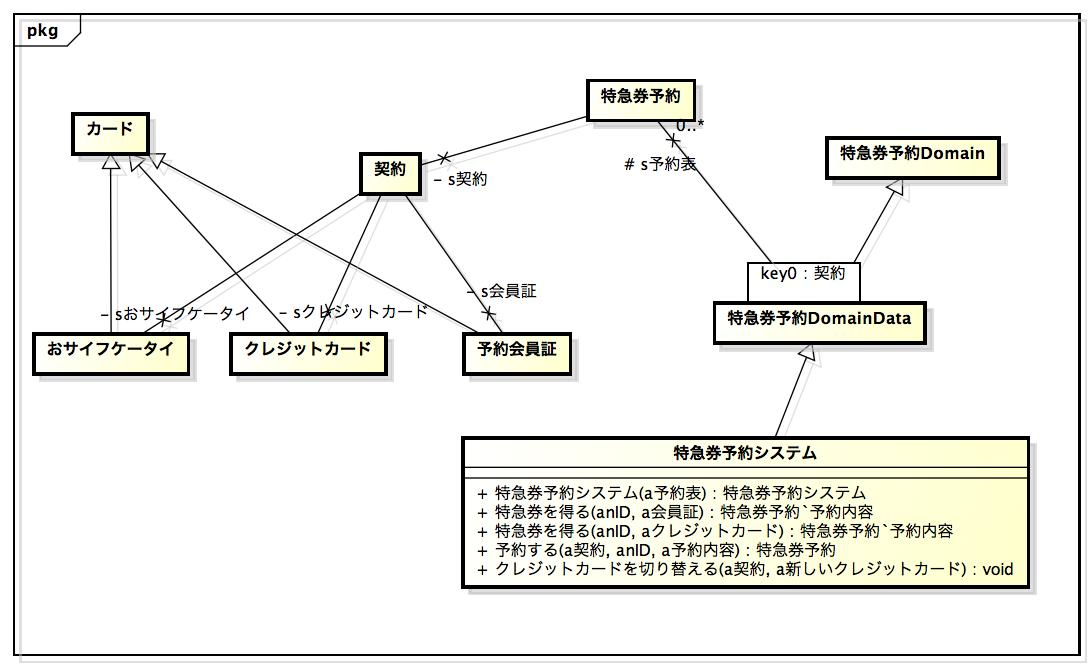
\includegraphics[width=55zw, keepaspectratio] {../EvolvedExpressReservation/image/ModifiedClassDiagram.jpg}}
%			\caption{修正後のクラス図}
%			\label{fig:ModifiedClassDiagram}
%			\index{しゆせいこのくらすす@修正後のクラス図}
%		\end{figure}
%
%		修正後のクラス図は、図\ref{fig:ModifiedClassDiagram}を参照のこと。

\subsection {特急券予約システムモデル化の統計情報}
\addcontentsline{toc}{section}{特急券予約システムモデル化の統計情報}
	\index{とっきゅうけんよやくしすてむもでるかのとうけいじょうほう@特急券予約システムモデル化の統計情報}
注釈抜きのVDM++ソース行数は、501行、
モデル作成工数は約1日、発表用の資料作成とVDM++モデルの読みやすさのための整形・清書に約2日、
モデルの修正工数は1日かかった。

なお、上記モデルの作成工数は、筆者が問題を解決するために消費した工数より少ない。